\documentclass[12pt,a4paper]{article}
\pdfminorversion=7

\usepackage[british]{babel}
\usepackage[a4paper,top=2cm,bottom=2cm,left=2.5cm,right=2.5cm,marginparwidth=1.75cm]{geometry}
\usepackage[style=apa,backend=biber]{biblatex}
\addbibresource{references.bib}
\DeclareLanguageMapping{british}{british-apa}
\DeclareFieldFormat[article]{volume}{\apanum{#1}}
\renewcommand*{\finalnamedelim}{%
  \ifnumgreater{\value{liststop}}{2}{\finalandcomma}{}%
  \addspace\&\space}

\usepackage{amsmath}
\usepackage{amssymb}
\usepackage{graphicx}
\usepackage[colorlinks=true,allcolors=blue]{hyperref}
\usepackage{booktabs}
\usepackage{threeparttable}
\usepackage{authblk}
\usepackage[T1]{fontenc}
\usepackage{csquotes}
\usepackage{url}
\usepackage{lmodern}
\usepackage{microtype}
\usepackage{setspace}
\usepackage{titlesec}
\usepackage{caption}
\usepackage{float}
\usepackage{lineno}
\onehalfspacing
\setlength{\emergencystretch}{3em}

\titleformat{\section}{\normalfont\Large\bfseries}{\thesection.}{1em}{}
\titleformat{\subsection}{\normalfont\large\bfseries}{\thesubsection.}{1em}{}
\captionsetup[table]{position=top,labelfont=bf}
\captionsetup[figure]{labelfont=bf}
\date{}

\begin{document}
\linenumbers

\begin{center}
{\LARGE\bfseries Cross-style robustness in image-to-3D generation is model-specific}
\\[1.2ex]
{\Large A paired four-model benchmark with known 3D ground truth}
\\[4ex]

{\large Wei Xiong$^{1}$, Wei Meng$^{2}$, Chu Qiu$^{4,*}$, ShuWen Li$^{1}$, and Zhanhao Liang$^{3,*}$}
\\[1.5ex]
{\small
$^{1}$Guilin Institute of Information Technology, No. 9 Yantu Road, Lingui District, Guilin, Guangxi 541100, China \\
$^{2}$Guilin Normal College, No. 9 Feihu Road, Lingui District, Guilin, Guangxi 541199, China \\
$^{3}$School of Materials Science and Engineering, South China University of Technology, Guangzhou, China \\
$^{4}$Guilin Life and Health Career Technical College, No. 1 Zhongyin West Road, Xiufeng District, Guilin, Guangxi 541001, China \\
$^{*}$Corresponding authors: Chu Qiu, \href{mailto:appamm94@gmail.com}{appamm94@gmail.com}; ORCID: \href{https://orcid.org/0009-0004-3523-5659}{0009-0004-3523-5659} \\
Zhanhao Liang, \href{mailto:lyon@cumt.edu.cn}{lyon@cumt.edu.cn}. \\
E-mail addresses: Wei Xiong, \href{mailto:xiongwei@guit.edu.cn}{xiongwei@guit.edu.cn};
Wei Meng, \href{mailto:mengwei@mail.glnc.edu.cn}{mengwei@mail.glnc.edu.cn};
ShuWen Li, \href{mailto:lishuwen@guit.edu.cn}{lishuwen@guit.edu.cn}.
}
\end{center}

\begin{abstract}
General-purpose image-to-3D systems are increasingly used with sketches and illustrations, but their geometric robustness outside photographic input remains unclear. We present a paired benchmark in which 120 public Google Scanned Objects are rendered from one fixed view as a photo-like reference and five matched abstractions: edge, flat colour, low detail, sketch, and watercolour. TripoSR, InstantMesh, Hunyuan3D 2.1, and TRELLIS are evaluated against repaired watertight ground truth using surface, solid-occupancy, topology, and independent six-view render diagnostics. The study comprises 6,240 successful reconstructions. A pre-specified robustness-gap statistic compares style-induced change in F-score@0.05 with change in voxel intersection over union. The proposed cross-model sketch effect was not confirmed: no model passed the 1\% Holm-corrected primary test, with mean gaps between $-0.0091$ and $0.0222$. However, the model-by-style interaction was strong ($p_{\mathrm{Holm}}=1.03\times10^{-8}$), and absolute degradation differed sharply. Under sketch input, InstantMesh lost 0.208 in F-score and 0.230 in voxel intersection over union, while mean changes for Hunyuan3D 2.1 and TRELLIS were small and their 99\% confidence intervals crossed zero. Six-view silhouette and normal-render diagnostics reproduced this contrast. View, severity, and seed analyses further showed that robustness rankings do not transfer unchanged across conditions. The results reject a universal surface--solid metric paradox and support a narrower conclusion: cross-style geometry robustness is a property of a model--style pairing. Evaluation and model selection for computational design should therefore include matched non-photographic inputs and report solid and multi-view diagnostics alongside surface scores.
\end{abstract}

\noindent\textbf{Keywords}: image-to-3D; artistic input; geometric robustness; paired benchmark; voxel IoU; computational design.

\section{Introduction}

Single-image 3D generation has become a practical route from a visual reference to an editable asset. Feed-forward reconstruction models and image-conditioned generative systems can now produce a mesh within seconds or minutes, reducing the amount of manual modelling needed for concept development, games, digital heritage, and design visualisation \parencite{hong2023lrm,tochilkin2024triposr,xu2024instantmesh,xiang2025trellis,hunyuan3d2025}. The input in these workflows is not always a photograph. Early design work often begins with a contour drawing, a flat-colour concept, a blurred thumbnail, or an illustration whose shading follows an artistic convention rather than physical illumination. A model that performs well on photographs may therefore encounter a different set of depth cues when used in the setting for which it is attractive.

Recent image-to-3D research has improved reconstruction speed, multi-view consistency, mesh quality, and material generation \parencite{liu2023zero123,liu2023one2345,liu2023one2345pp,long2023wonder3d,long2025wonder3dpp,wang2024crm,wei2024meshlrm,wu2024unique3d,liu2024meshformer,wang2025mage}. This progress does not by itself establish robustness to visual abstraction. A sketch preserves some cues, such as object boundary and part arrangement, while weakening texture, shading, and fine-scale appearance. An edge image removes most interior evidence. Flat colour preserves regions but compresses reflectance and illumination. Watercolour changes local contrast and boundary sharpness. These transformations can alter the evidence used by an image-conditioned model even when object identity, camera, foreground mask, and framing are unchanged.

The evaluation problem is equally important. Chamfer distance and thresholded F-score are widely used because they provide reproducible comparisons between sampled surfaces. They do not directly measure whether a reconstruction occupies the correct solid region, remains connected, or has plausible appearance under unseen views. A thin or fragmented reconstruction can place many sampled points near the reference surface while failing as a three-dimensional asset. Conversely, an occupancy score can penalise a mesh for a local solid difference that has limited visual effect. Neither family should be treated as a complete substitute for the other. The relevant question is whether they respond consistently to a controlled change in input style.

Work on sketch-to-3D and stylised reconstruction has demonstrated that non-photographic input is a substantive task rather than a cosmetic variation \parencite{sanghi2023sketchashape,chen2023panic3d,zheng2024sketch3d,zhou2024drawingspinup,lee2025pasta,cong2025art3d}. Most studies in this line introduce a method for one artistic domain. Fewer studies ask how several general-purpose systems respond when exactly the same object and view are presented through different depictions. Unpaired collections of photographs and artworks cannot answer this cleanly because style is confounded with category, pose, geometry, and image source. Human ratings of recognisability are also difficult to interpret when the input and output do not represent the same object, a problem that motivated the controlled design used here.

We study cross-style robustness with known 3D ground truth. The confirmatory cohort contains 120 objects from Google Scanned Objects (GSO) \parencite{downs2022gso}. Each object contributes one photo-like rendering and five deterministic abstractions under the same orthographic camera. Four open image-to-3D systems process these matched inputs: TripoSR \parencite{tochilkin2024triposr}, InstantMesh \parencite{xu2024instantmesh}, Hunyuan3D 2.1 \parencite{hunyuan3d2025}, and TRELLIS \parencite{xiang2025trellis}. Every prediction is compared with a watertight solid reconstructed from the source scan. One model-level alignment is calibrated on a separate discovery set, and per-sample scaling is prohibited. The design therefore isolates input depiction as far as the available systems permit.

The study began with a specific proposition raised by a separate 30-object discovery experiment: stylised input might create a surface--solid robustness gap, in which F-score understates degradation in solid occupancy. We froze a primary statistic before selecting the confirmatory objects, rendering their inputs, or running the four systems. For object $i$, model $m$, and style $s$, the robustness gap is
\begin{equation}
\mathrm{RG}_{i,m,s}
=
\left(F_{i,m,s}-F_{i,m,p}\right)
-
\left(I_{i,m,s}-I_{i,m,p}\right),
\label{eq:intro_rg}
\end{equation}
where $p$ denotes the paired photo condition, $F$ is F-score@0.05, and $I$ is voxel intersection over union (IoU). Positive RG means that occupancy deteriorates more than the surface score indicates.

The primary cross-model proposition did not survive confirmation. No model passed the Holm-corrected 1\% sketch test. The near-zero result should not, however, be read as evidence that style is harmless. The four systems responded very differently. InstantMesh underwent large surface, occupancy, topology, and six-view rendering losses for sketch and edge inputs. TripoSR showed smaller but detectable losses in several diagnostics. Hunyuan3D 2.1 and TRELLIS were comparatively stable for the canonical sketch condition, although their results varied under other styles, viewpoints, and random seeds. A cluster-robust model-by-style interaction was significant for the primary RG definition. The evidence therefore changes the paper's claim: there is no universal metric paradox across these systems, but there is a strong model--style dependency that an evaluation based only on photographs would miss.

The paper makes four contributions. First, it introduces a paired, known-ground-truth protocol that holds object, view, mask, framing, and style-generation procedure fixed across four image-to-3D systems. Second, it reports a complete 6,240-reconstruction comparison using surface, solid, topology, and independent render-space diagnostics. Third, it tests and rejects a pre-specified universal sketch robustness-gap proposition rather than replacing it with a favourable post hoc claim. Fourth, it identifies where the practically important degradation lies: not in a common gap shared by all models, but in model-specific responses that are only partly stable across seed, viewpoint, and abstraction severity.

This evidence answers three questions. How do five controlled abstractions change the geometry recovered by four current image-to-3D systems? Does a surface--solid gap found during discovery replicate across models? Which robustness checks help distinguish a systematic response from a particular camera, random seed, or metric threshold? The answers matter for computational design because choosing an image-to-3D model by its photographic examples alone can conceal large losses under the depictions used during actual concept work.

\section{Related work}

\subsection{Single-image 3D reconstruction}

The current generation of image-to-3D systems draws on view-conditioned diffusion, large reconstruction models, and large-scale collections of rendered 3D objects. Zero-1-to-3 learns relative-camera-conditioned novel views from a single image \parencite{liu2023zero123}. One-2-3-45 and One-2-3-45++ combine multi-view generation with fast 3D reconstruction \parencite{liu2023one2345,liu2023one2345pp}. Wonder3D uses cross-domain diffusion to generate consistent normal and colour views, with later work improving fidelity \parencite{long2023wonder3d,long2025wonder3dpp}. These systems helped establish a pipeline in which learned view generation supplies evidence for subsequent geometry recovery.

Large reconstruction models move more of the inference into a feed-forward network. LRM demonstrated scalable transformer-based reconstruction from a single image \parencite{hong2023lrm}. TripoSR reduced the cost of this approach and made fast open inference widely accessible \parencite{tochilkin2024triposr}. InstantMesh combines a sparse-view reconstruction model with generated multi-view images \parencite{xu2024instantmesh}. CRM, MeshLRM, Unique3D, MeshFormer, LRM-Zero, GeoLRM, multi-view LRM, and GS-LRM extend this family through convolutional reconstruction, direct mesh prediction, synthetic training data, or geometry-aware representations \parencite{wang2024crm,wei2024meshlrm,wu2024unique3d,liu2024meshformer,xie2024lrmzero,zhang2024geolrm,li2024mvlrm,zhang2024gslrm}. Hunyuan3D 2.1 and TRELLIS represent more recent high-capacity systems with shape and material pipelines or structured 3D latent representations \parencite{hunyuan3d2025,xiang2025trellis}.

Training and evaluation in this area depend on large 3D corpora. Objaverse and Objaverse-XL expanded the scale of available object assets \parencite{deitke2022objaverse,deitke2023objaversexl}, while later curation work has added quality annotations \parencite{lin2025objaversepp}. GSO is much smaller but offers high-quality scanned household objects with textured geometry \parencite{downs2022gso}. The present work uses GSO because the experimental question requires inspectable object-level geometry and a reproducible route to solid ground truth, not because it covers every design category.

Most reported comparisons emphasise natural or rendered photo-like images. This is appropriate for measuring core reconstruction quality, but it leaves an operational gap. A designer may select a model based on a photographic benchmark and then use it with a sketch or flat illustration. The resulting distribution shift is structured: semantic content and silhouette can remain stable while cues to thickness and back-side geometry change. Our benchmark measures this shift directly rather than treating non-photographic inputs as anecdotal examples.

\subsection{Sketches and artistic inputs}

Sketch-based modelling has a long history, and recent generative methods have expanded it to zero-shot and text-aligned shape generation. Sketch-A-Shape generates 3D shapes from sketches without task-specific examples \parencite{sanghi2023sketchashape}; Sketch3D introduces style-consistent guidance \parencite{zheng2024sketch3d}; and PASTA incorporates part-aware priors \parencite{lee2025pasta}. A recent survey documents the breadth of deep sketch-based 3D modelling and the continuing difficulty of interpreting sparse or ambiguous strokes \parencite{tono2026sketchsurvey}.

Other studies focus on particular visual domains. PAniC-3D reconstructs stylised anime portraits \parencite{chen2023panic3d}. DrawingSpinUp targets animation from a single character drawing \parencite{zhou2024drawingspinup}. Art3D addresses flat-coloured illustration with a training-free correction pipeline \parencite{cong2025art3d}. Work on manuscript miniatures examines reconstruction from historical illustrations \parencite{pallotto2026miniatures}, and recent methods also study stylisation of reconstructed assets or language-driven artistic scenes \parencite{oztas2025stylizationlrm,li2025artiscene}.

These contributions show that artistic input needs specialised treatment, but they do not provide a controlled comparison of general-purpose systems across several abstractions of the same object. Real artworks differ in drawing skill, semantic exaggeration, perspective, composition, and background. That diversity is valuable for ecological evaluation, but it makes causal interpretation difficult. Controlled transformations provide a complementary diagnostic. They are not substitutes for human artwork; they are interventions that retain the object, camera, and foreground support while altering selected appearance cues.

The distinction also changes the role of human evaluation. When an artwork and a generated mesh are only loosely related, a rater may be unable to decide whether disagreement reflects poor reconstruction, artistic freedom, or a mismatched sample. A known-object paired design supplies a geometric target and makes human inspection interpretable. The current study stops short of a human usability experiment, but its inputs and outputs are organised so that such an experiment can compare matched cases rather than unrelated pictures.

\subsection{Evaluation of generated 3D assets}

Evaluation has become a research problem in its own right. 3DGen-Bench proposes a broad benchmark suite for generative 3D systems \parencite{jiang2025threedgenbench}, and 3D Arena supports comparative evaluation of generated assets \parencite{ebert2025threedarena}. SI23DCQA studies perceptual quality assessment for single-image-to-3D content \parencite{fu2025si23dcqa}. Cue3D examines how image cues contribute to single-image 3D generation \parencite{li2025cue3d}. In adjacent design research, CADBench evaluates generated programmes and geometric outputs with criteria beyond a single visual score \parencite{doris2026cadbench}.

Surface distance remains central because it is objective and widely implemented. Chamfer distance measures average nearest-neighbour discrepancy between sampled surfaces. Thresholded precision, recall, and F-score measure how much of one surface lies within a tolerance of the other. These metrics are sensitive to alignment, sampling, and threshold, but they provide useful geometric evidence. Solid occupancy, topology, and multi-view rendering answer different questions. Voxel IoU asks whether predicted and reference shapes occupy the same region. Connected-component and boundary-edge counts expose fragmentation or open surfaces. Silhouette and normal-render similarities test whether errors remain visible when the object is observed from several standardised directions.

Our use of a robustness gap is not a proposal to replace one metric with another. It is a test of disagreement between metric families under a paired input intervention. If the gap had replicated across models, a surface-only benchmark would have had a systematic blind spot. Its failure to replicate leads to a more useful conclusion: the disagreement itself depends on architecture and style. This result supports multi-metric reporting while warning against treating any one gap statistic as universal.

\section{Material and methods}

\subsection{Study design and frozen evidence boundary}

The experiment was divided into discovery and confirmation. A 30-object pilot, denoted D30, was used to formulate the robustness-gap hypothesis, estimate a conservative effect size, and calibrate one alignment transform per model. All D30 objects and outputs were excluded from confirmatory tests. Before selecting confirmatory objects, generating their styled inputs, or running model inference, we froze the cohort-selection rule, ground-truth admission thresholds, models, main styles, robustness subsets, metrics, primary statistic, bootstrap procedure, multiplicity correction, and publication evidence gate.

The frozen gate required the sketch RG 99\% confidence interval to lie above zero in at least two of four models after Holm correction at $\alpha=0.01$. It also required at least two of four supporting criteria concerning seed direction, view direction, severity slope, and model-by-style interaction. The gate was intentionally stricter than a single uncorrected positive estimate. With 120 independent objects, a two-sided $\alpha=0.01$, and a pilot effect shrunk to a paired standardised mean of 0.35, the normal approximation gave about 90\% power for a model-specific test. Repeated seeds, styles, and views were not counted as additional independent objects.

Figure~\ref{fig:framework} summarises the paired protocol. The design uses the same reference geometry to generate every depiction, sends each depiction through four fixed systems, and evaluates each output with a common set of diagnostics. The primary comparison is within object and model. This avoids attributing category or camera differences to style.

\begin{figure}[!ht]
\centering
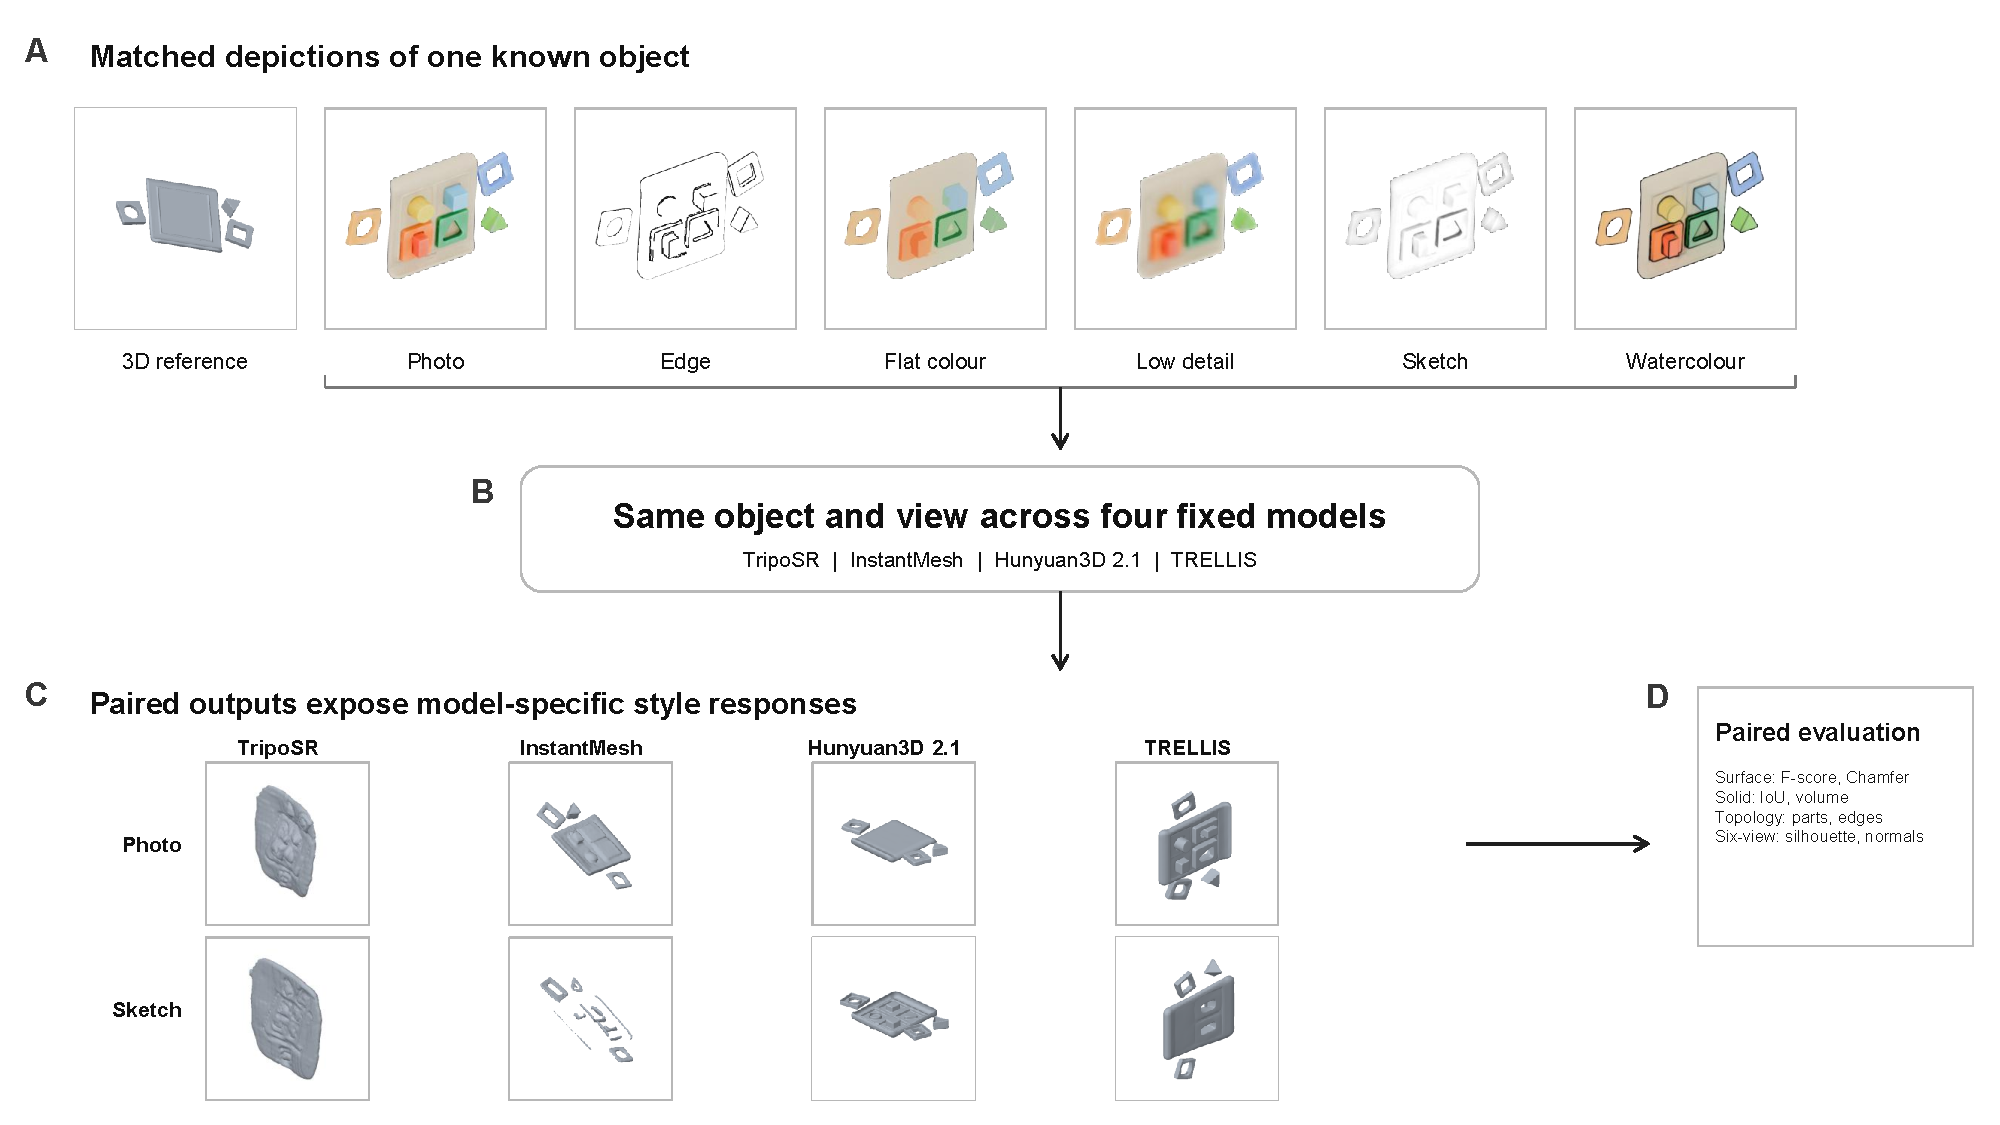
\includegraphics[width=\linewidth]{figures/fig1_confirmatory_framework.pdf}
\caption{\label{fig:framework}Paired four-model evaluation protocol, illustrated with object c120\_017. (A) One known 3D object supplies a photo-like rendering and five matched abstractions under the same orthographic view and foreground mask. (B) The inputs are processed without style-specific tuning by TripoSR, InstantMesh, Hunyuan3D 2.1, and TRELLIS. (C) Photo and sketch outputs from the four systems show that the response to the same depiction shift is model-specific. (D) Surface, solid, topology, and independent six-view diagnostics are computed against the repaired 3D reference. The displayed meshes and inputs are experimental outputs rather than AI-drawn placeholders.}
\end{figure}

\subsection{Confirmatory objects and solid ground truth}

The confirmatory cohort C120 was drawn from public GSO assets \parencite{downs2022gso}. Candidate order was fixed by the SHA-256 rank of a project identifier concatenated with the object name. Processing followed that order until 120 objects not present in D30 passed the solid-ground-truth audit. Model outputs were unavailable during selection. Branded object names were permitted in numerical analysis, but neutral objects were chosen for publication figures.

Each source asset retained its textured GLB for input rendering. Triangle geometry was concatenated and normalised to unit maximum extent for evaluation. The source was then converted to a solid with ManifoldPlus at official commit \texttt{a0cc6d9} and depth 8 \parencite{huang2020manifoldplus}. A repaired object was admitted only if it was watertight, winding-consistent, and a positive-volume solid with at most four connected components. The repair also had to preserve the source surface: F-score@0.02 of at least 0.95, bidirectional surface-distance 95th percentile no greater than 0.02, symmetric Chamfer-L2 no greater than 0.0002, and mean absolute relative extent error no greater than 0.03. No threshold was revised after model results became available.

This repair step was necessary because solid occupancy cannot be defined consistently for open triangle soups. It was not used to make the target easier for a particular model. The admission tests require the repaired solid to remain close to the original scan, and all four systems are evaluated against the same repaired target. Source and repaired identifiers, audit values, and hashes are retained in the reproducibility package.

\subsection{Matched depictions}

For every C120 object, the canonical condition was a 512$\times$512 photo-like rendering of the textured scan on a white background. The camera was orthographic and used the frozen D30 transform. Five deterministic abstractions were derived from this rendering:
\begin{itemize}
    \item \textbf{edge}, which retains high-contrast contours and removes most interior appearance;
    \item \textbf{flat colour}, which simplifies local colour and shading while retaining foreground regions;
    \item \textbf{low detail}, which suppresses fine texture and high-frequency structure;
    \item \textbf{sketch}, which uses a greyscale colour-dodge construction to emphasise drawn contours; and
    \item \textbf{watercolour}, which softens boundaries and local contrast while retaining broad colour variation.
\end{itemize}

The exact photo alpha mask was attached to every abstraction. Object scale, framing, camera, output resolution, and white background were therefore identical within a matched set. The terms \enquote{photo} and \enquote{style} refer to these controlled rendering conditions; the photo condition is not a photograph captured in an uncontrolled real scene. The transforms were generated before inference and were not revised in response to model behaviour.

Two robustness subsets used the first 30 C120 objects under the frozen hash rank. The view subset V30 added fixed world-y rotations of $-30^{\circ}$ and $+30^{\circ}$ to the canonical camera and rendered photo, edge, and sketch conditions. The severity subset S30 used edge and sketch transformations at low, medium, and high levels. Medium was identical to the main condition. Low severity blended 35\% of the medium abstraction with 65\% of the photo foreground. High edge used stronger Canny thresholds and dilation; high sketch used a broader colour-dodge blur followed by downsampling and upsampling. Severity was encoded as 0, 1, and 2 for the pre-specified linear trend.

\subsection{Reconstruction systems and inference schedule}

We evaluated four open systems with fixed official code revisions. TripoSR used commit \texttt{107cefd} and \texttt{stabilityai/TripoSR} weights, marching-cubes resolution 128, and chunk size 4096 \parencite{tochilkin2024triposr}. It is deterministic under this pipeline. InstantMesh used commit \texttt{08822c5}, the \texttt{instant-mesh-large} configuration, Zero123Plus v1.2 for multi-view generation, and 75 diffusion steps \parencite{xu2024instantmesh}. Hunyuan3D 2.1 used commit \texttt{82920d6}, 25 shape-generation steps, and octree resolution 384 \parencite{hunyuan3d2025}. TRELLIS used commit \texttt{442aa1e} with \texttt{microsoft/TRELLIS-image-large}, 25 sparse-structure steps, 25 structured-latent steps, classifier-free guidance 5.0, and mesh decoding \parencite{xiang2025trellis}. Texture generation was not used because the primary endpoints concern geometry.

InstantMesh, Hunyuan3D 2.1, and TRELLIS were run with paired seeds 20260715 and 3407 for the C120 main experiment. The primary seed 20260715 was used for V30 and the additional low/high S30 conditions; medium severity reused the corresponding main output. TripoSR contributed 1,020 deterministic reconstructions. Each stochastic model contributed 1,740 reconstructions. All 6,240 scheduled jobs produced an output and entered the evaluation. Table~\ref{tab:design} separates the main and robustness workloads.

\begin{table}[!ht]
\caption{\label{tab:design}Confirmatory design and completed inference workload. Main inputs contain the photo condition and five abstractions. V30 contains two additional views for photo, edge, and sketch. S30 adds low and high edge/sketch conditions; medium reuses the main output.}
\centering
\begin{threeparttable}
\small
\begin{tabular}{lrrrrr}
\toprule
System & Objects & Seeds & Main jobs & Robustness & Total \\
\midrule
TripoSR & 120 & deterministic & 720 & 300 & 1,020 \\
InstantMesh & 120 & 2 & 1,440 & 300 & 1,740 \\
Hunyuan3D 2.1 & 120 & 2 & 1,440 & 300 & 1,740 \\
TRELLIS & 120 & 2 & 1,440 & 300 & 1,740 \\
\midrule
Total & 120 & -- & 5,040 & 1,200 & 6,240 \\
\bottomrule
\end{tabular}
\begin{tablenotes}\footnotesize
\item The independent six-view render diagnostic was computed for all 5,040 main-condition meshes.
\end{tablenotes}
\end{threeparttable}
\end{table}

Inference ran on one NVIDIA GeForce RTX 5090 with 32 GB memory under PyTorch 2.8.0 and CUDA 12.8. Compatibility changes for TRELLIS were restricted to dependencies and did not alter weights, samplers, guidance values, step counts, sparse resolution, or mesh decoding. Code commit, weight identifier, environment, schedule hash, and per-job status were recorded for every model.

\subsection{Model-level alignment}

Image-to-3D systems use different coordinate conventions and output scales. We therefore calibrated one fixed similarity transform per model using ten photo reconstructions from D30 only. For each calibration object, the candidate scale was the ratio between the largest ground-truth extent and the largest predicted extent. The model-level scale was the median of these ten ratios. We searched all 48 signed-axis permutations and selected the one with the lowest median symmetric Chamfer-L2 across the ten discovery objects after application of the single model-level scale.

For confirmatory evaluation, only translation was removed per sample. Per-sample rescaling, axis search, iterative closest point alignment, and non-rigid registration were forbidden. This constraint is important. An unconstrained per-object scale fit could hide the depth or occupancy changes that the benchmark is designed to detect. The fixed transform also prevents C120 results from influencing calibration.

\subsection{Surface, solid, topology, and render metrics}

Surface metrics used 10,000 area-weighted samples from each prediction and reference, with deterministic hash-derived sampling seeds. Let $P$ and $G$ be the predicted and ground-truth point sets. Symmetric Chamfer-L2 was
\begin{equation}
\mathrm{CD}(P,G)
=
\frac{1}{|P|}\sum_{p\in P}\min_{g\in G}\|p-g\|_2^2
+
\frac{1}{|G|}\sum_{g\in G}\min_{p\in P}\|g-p\|_2^2.
\label{eq:chamfer}
\end{equation}
At tolerance $\tau$, surface precision and recall were the fractions of $P$ and $G$ whose nearest neighbour lay within $\tau$. Their harmonic mean gave
\begin{equation}
F_{\tau}
=
\frac{2\,\mathrm{Prec}_{\tau}\,\mathrm{Rec}_{\tau}}
{\mathrm{Prec}_{\tau}+\mathrm{Rec}_{\tau}}.
\label{eq:fscore}
\end{equation}
We report $F_{0.05}$ as the primary surface score, $F_{0.10}$ as a threshold sensitivity analysis, Chamfer-L2, and normal consistency.

Solid occupancy used a filled $128^3$ voxel grid with fixed extent 1.5. If $V_P$ and $V_G$ are the occupied voxel sets,
\begin{equation}
\mathrm{IoU}(V_P,V_G)
=
\frac{|V_P\cap V_G|}{|V_P\cup V_G|}.
\label{eq:iou}
\end{equation}
We also recorded solid volume, per-axis extents, and depth error. Raw-mesh topology was measured before alignment through watertightness, winding consistency, component count, boundary edges, and non-manifold edges.

An independent render-space diagnostic used six standard views at 256$\times$256 resolution. It compared predicted and reference silhouette IoU and normal-render similarity. These views were not used for input generation or geometric alignment. They test whether a paired degradation remains visible beyond the source view and beyond the point/voxel implementations.

For style $s$ relative to photo $p$, the paired changes were
\begin{align}
\Delta F_{i,m,s} &= F_{i,m,s}-F_{i,m,p}, \\
\Delta I_{i,m,s} &= I_{i,m,s}-I_{i,m,p}.
\end{align}
Equation~\ref{eq:intro_rg} is equivalently $\mathrm{RG}=\Delta F-\Delta I$. We also report surface degradation $D_F=-\Delta F$ and solid degradation $D_I=-\Delta I$, so positive values denote loss in both families. RG is their difference, $D_I-D_F$. A positive value does not imply that the surface score improved; it means only that solid occupancy deteriorated more.

\subsection{Statistical analysis}

The independent unit was the object. For stochastic systems, seeds were averaged within object before the primary analysis. Model-specific mean sketch RG was estimated with 50,000 object-cluster bootstrap resamples, a fixed bootstrap seed of 20260715, two-sided 99\% confidence intervals, and two-sided bootstrap $p$-values. Holm's procedure corrected the four model-specific primary tests. The same analysis at $F_{0.10}$ was labelled sensitivity rather than an alternative primary endpoint.

To test heterogeneity, we fitted $\mathrm{RG}\sim\mathrm{model}\times\mathrm{style}$ to the 2,400 object-averaged style records and used an object-cluster-robust joint Wald test for the 12 interaction terms. Primary-threshold and sensitivity-threshold interaction tests were corrected together. Absolute $\Delta F$, $\Delta I$, topology changes, and render-space changes were secondary endpoints with 99\% object-bootstrap intervals.

V30 paired each style output with the photo output from the same object, model, seed, and view. S30 estimated an object-cluster bootstrap slope across ordered severity levels. Seed reliability was assessed through Pearson correlation, Spearman correlation, and sign agreement of object-level sketch RG. Morphology associations used Spearman correlation between sketch RG and seven ground-truth shape descriptors, with Holm correction within model. They were specified as exploratory and are not interpreted causally.

Three representative sketch cases in Figure~\ref{fig:cases} were selected by a frozen rule after the numerical analysis: a high positive-gap case, a moderate positive-gap case, and a negative-gap case near pre-defined targets. The selection used metric values rather than visual preference. The figure includes input, ground truth, photo output, sketch output, case identifier, model, seed, and paired metric changes.

\section{Results}

\subsection{Execution completeness and photographic baselines}

All 6,240 scheduled reconstructions completed, and all 5,040 main-condition meshes received six-view render diagnostics. There were no silent exclusions from the primary object-level table. The four models nevertheless began from different photographic baselines (Table~\ref{tab:photo}). InstantMesh had the highest mean $F_{0.05}$ (0.381), voxel IoU (0.264), and normal consistency (0.609), and the lowest Chamfer-L2 (0.0365). Hunyuan3D 2.1 was close on these measures. TripoSR produced the highest watertight fraction but lower surface and occupancy scores. TRELLIS had the lowest mean photo IoU (0.159) while retaining moderate surface scores.

\begin{table}[!ht]
\caption{\label{tab:photo}Mean photo-condition geometry before style perturbation ($n=120$ objects per model). Lower Chamfer-L2 is better; all other reported quality metrics are higher-is-better.}
\centering
\begin{threeparttable}
\begin{tabular}{lrrrrrr}
\toprule
System & $F_{0.05}$ & $F_{0.10}$ & Voxel IoU & Chamfer-L2 & Normal cons. & Watertight \\
\midrule
TripoSR & 0.289 & 0.502 & 0.180 & 0.0489 & 0.496 & 1.000 \\
InstantMesh & 0.381 & 0.610 & 0.264 & 0.0365 & 0.609 & 0.983 \\
Hunyuan3D 2.1 & 0.355 & 0.588 & 0.244 & 0.0388 & 0.594 & 0.996 \\
TRELLIS & 0.302 & 0.515 & 0.159 & 0.0470 & 0.548 & 0.967 \\
\bottomrule
\end{tabular}
\begin{tablenotes}\footnotesize
\item Stochastic-model values are averaged across the two paired seeds within object.
\end{tablenotes}
\end{threeparttable}
\end{table}

These baseline differences matter for interpretation. A model with a stronger photo reconstruction has more quality to lose under style perturbation, whereas a weaker baseline can occasionally improve after simplification of the input. The paired design controls the comparison within each model; it does not assume that the four photo baselines are interchangeable.

\subsection{The pre-specified cross-model sketch gap was not confirmed}

Figure~\ref{fig:mainresults} and Table~\ref{tab:primary} report the primary result. TripoSR had a small positive mean sketch RG of 0.0089 with a 99\% interval that narrowly excluded zero, but its raw $p=0.00944$ became $p_{\mathrm{Holm}}=0.0378$. InstantMesh had the largest mean, 0.0222, but substantial object variation produced a 99\% interval of $[-0.0124,0.0583]$. Hunyuan3D 2.1 and TRELLIS had small negative means with intervals crossing zero. No model passed the corrected 1\% criterion, so the required count was 0/4 rather than at least 2/4.

\begin{table}[!ht]
\caption{\label{tab:primary}Pre-specified primary test of the sketch surface--solid robustness gap. Positive RG means voxel-IoU degradation exceeds F-score@0.05 degradation. Confidence intervals use 50,000 object-cluster bootstrap resamples.}
\centering
\begin{tabular}{lrrrrc}
\toprule
System & Mean RG & 99\% CI & Raw $p$ & Holm $p$ & Pass \\
\midrule
TripoSR & 0.0089 & [0.0001, 0.0180] & 0.0094 & 0.0378 & No \\
InstantMesh & 0.0222 & [$-0.0124$, 0.0583] & 0.1028 & 0.3083 & No \\
Hunyuan3D 2.1 & $-0.0041$ & [$-0.0114$, 0.0030] & 0.1445 & 0.3083 & No \\
TRELLIS & $-0.0091$ & [$-0.0256$, 0.0071] & 0.1470 & 0.3083 & No \\
\bottomrule
\end{tabular}
\end{table}

\begin{figure}[!ht]
\centering
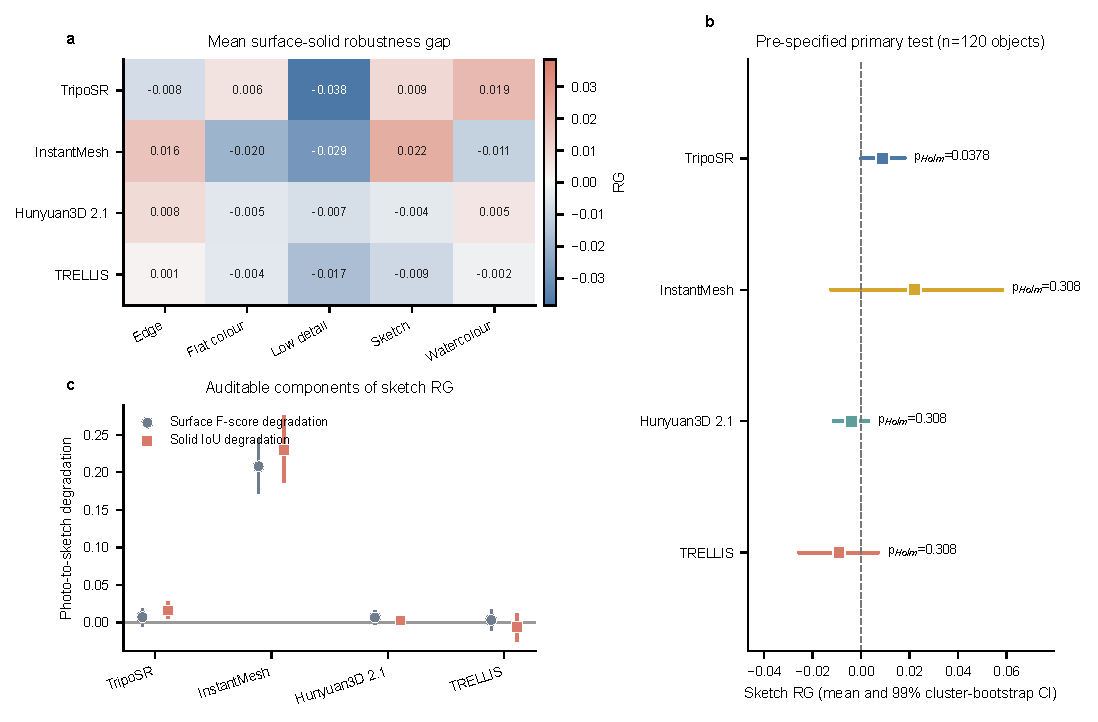
\includegraphics[width=\linewidth]{figures/fig2_confirmatory_main.pdf}
\caption{\label{fig:mainresults}Main quantitative results. (A) Mean RG for all 20 model--style pairs. The sign and magnitude vary across both axes. (B) Mean sketch RG and 99\% object-cluster bootstrap intervals for the pre-specified four-model primary test; labels show Holm-adjusted $p$-values. No model passes the corrected 1\% threshold. (C) The two auditable components of sketch RG. InstantMesh loses substantially in both F-score and voxel IoU, whereas mean losses for Hunyuan3D 2.1 and TRELLIS are close to zero.}
\end{figure}

The supporting publication gate also failed. Only one of four supporting criteria passed. InstantMesh was the only stochastic model with a positive mean sketch RG under both seeds, fewer than the two required. No model had positive mean sketch RG at both additional V30 views. Only TRELLIS had a positive sketch severity slope. The model-by-style interaction was the sole passing support item. The confirmatory evidence therefore does not justify the discovery-stage claim that a positive sketch gap is shared across image-to-3D systems.

The threshold sensitivity reinforces the need for restraint. At $F_{0.10}$, the model-by-style interaction had $p_{\mathrm{Holm}}=0.0586$, compared with $1.03\times10^{-8}$ at $F_{0.05}$. The primary conclusion is not reversed because the primary endpoint was fixed, but the contrast shows that the apparent metric-family disagreement depends partly on how surface agreement is operationalised.

\subsection{Style response is strongly model-specific}

Failure of the universal gap does not imply a common null response. The object-cluster-robust interaction at the primary threshold was strong ($\chi^2_{12}=63.51$, $p_{\mathrm{Holm}}=1.03\times10^{-8}$). Figure~\ref{fig:mainresults}A shows why. TripoSR's mean RG ranged from $-0.038$ for low detail to 0.019 for watercolour. InstantMesh ranged from $-0.029$ for low detail to 0.022 for sketch. Hunyuan3D 2.1 remained within approximately $\pm0.008$ across all styles. TRELLIS means were non-positive except for a near-zero edge result.

These signs have to be read together with absolute degradation. A near-zero RG can occur because neither metric changes, or because both change by a similar amount. InstantMesh sketch is the second case. Mean $F_{0.05}$ fell by 0.208 (99\% CI $[-0.244,-0.173]$), and voxel IoU fell by 0.230 (99\% CI $[-0.274,-0.189]$). Its mean RG was only 0.022 because both metric families recorded a large failure. Edge was similarly damaging: $\Delta F_{0.05}=-0.231$ and $\Delta\mathrm{IoU}=-0.246$. A gap-only report would understate this practical loss.

TripoSR showed smaller but non-trivial changes. For sketch, the $F_{0.05}$ interval crossed zero ($\Delta F=-0.007$, 99\% CI $[-0.017,0.004]$), but $F_{0.10}$ fell by 0.022 and voxel IoU fell by 0.016, with both 99\% intervals below zero. Watercolour reduced voxel IoU by 0.024 while its $F_{0.05}$ change was close to zero, producing the model's largest positive mean RG. Low-detail input had the opposite pattern: mean voxel IoU increased by 0.028 while $F_{0.05}$ decreased by 0.010, yielding a negative RG of $-0.038$.

Hunyuan3D 2.1 was stable under canonical sketch input: $\Delta F_{0.05}=-0.0064$ and $\Delta\mathrm{IoU}=-0.0024$, with both 99\% intervals crossing zero. It was less stable for edge and low detail. Edge reduced $F_{0.05}$ by 0.030 and IoU by 0.038; low detail reduced them by 0.039 and 0.032. TRELLIS showed a related pattern. Canonical sketch changes were small, but edge reduced $F_{0.05}$ by 0.051 and IoU by 0.052, and low detail reduced them by 0.047 and 0.030. Thus the two newer systems were not uniformly invariant to abstraction. Their strongest perturbation differed from the discovery-stage focus on sketch.

Topology added another distinction. InstantMesh sketch outputs contained, on average, 22.5 more connected components than their paired photo outputs, consistent with fragmentation in the most severe cases. TripoSR gained 1.2 components on average, while Hunyuan3D 2.1 and TRELLIS had small mean component changes. TRELLIS lost 5.4 percentage points in watertightness under sketch, despite its near-zero surface and occupancy means. The topology result is secondary, but it illustrates why an apparently stable pair of fidelity scores does not certify an editable mesh.

\subsection{Object-level cases explain both positive and negative gaps}

Figure~\ref{fig:cases} separates object-level variation from model means. InstantMesh occupies the widest range of surface and solid degradation, including many cases in which both are severe. TripoSR and Hunyuan3D 2.1 cluster more tightly around the origin for sketch. TRELLIS includes positive and negative outliers despite its small mean. The diagonal is an equality line: points above it have positive RG, and points below it have negative RG.

\begin{figure}[H]
\centering
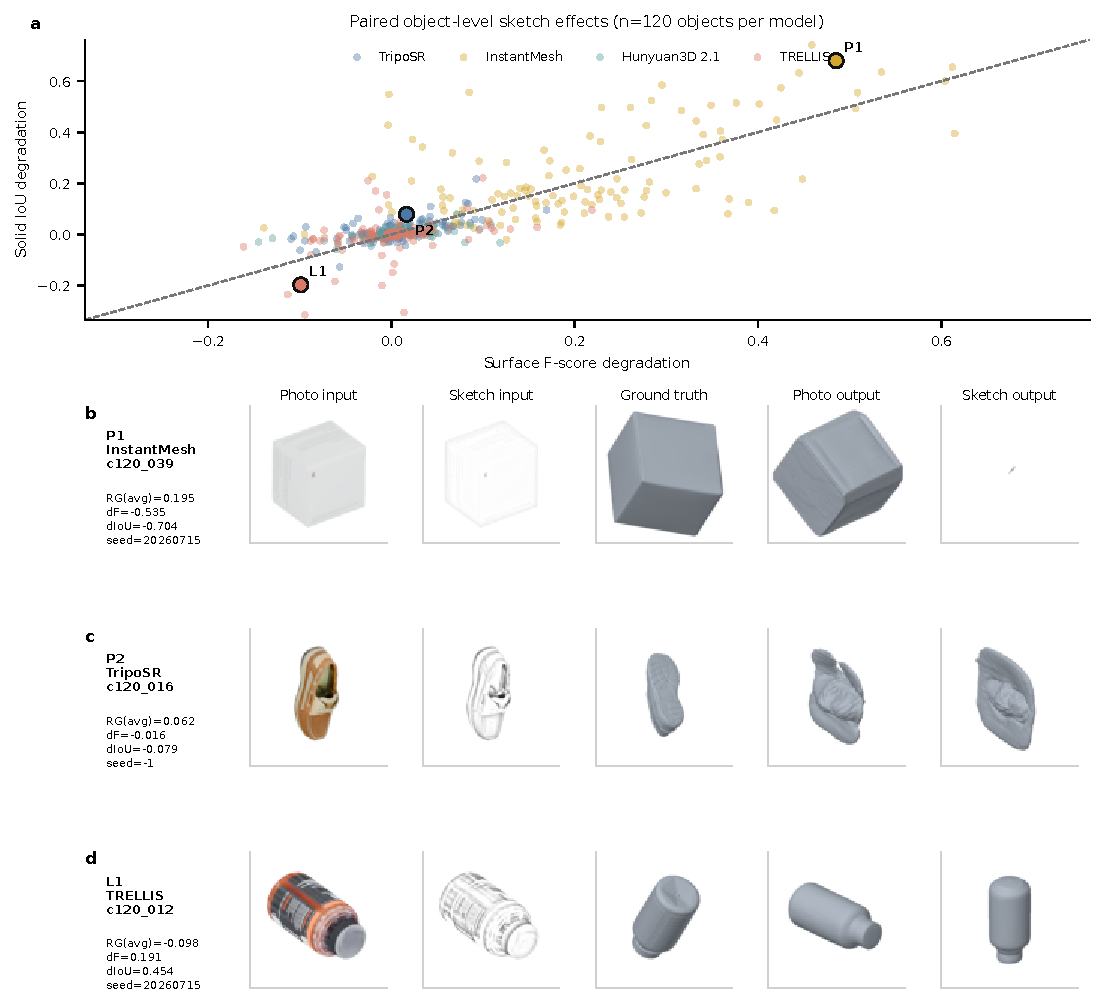
\includegraphics[width=\linewidth]{figures/fig3_confirmatory_cases.pdf}
\caption{\label{fig:cases}Object-level sketch effects and representative cases. (A) Surface F-score degradation versus voxel-IoU degradation for 120 objects per model. The dashed diagonal marks equal degradation; distance above it is positive RG. P1, P2, and L1 were selected by a frozen metric-based rule. (B) P1 is an InstantMesh failure in which the sketch output nearly disappears ($\Delta F=-0.535$, $\Delta\mathrm{IoU}=-0.704$, RG=0.195). (C) P2 shows a modest positive TripoSR gap with similar-looking source-view meshes. (D) L1 is a negative-gap TRELLIS case: the sketch output changes substantially, yet voxel IoU increases more than F-score. These examples show why RG sign, absolute fidelity, and visual geometry must be interpreted together.}
\end{figure}

P1 demonstrates that a positive gap can accompany an obvious failure in both metric families. The sketch depiction retains the broad cuboid outline, but InstantMesh produces almost no usable geometry. P2 is less dramatic: TripoSR's sketch output remains recognisable, while the solid score falls more than the surface score. L1 prevents a one-sided visual narrative. TRELLIS changes the pose and proportions of a cylindrical object, but its voxel IoU increases by 0.454 while F-score increases by 0.191, giving a negative RG. The output is not necessarily a better design asset; it is simply an example where occupancy benefits more under the chosen alignment and grid.

The figure also clarifies why human rating must use matched targets. The photo and sketch inputs in each row represent the same object and camera, and both outputs can be compared with a displayed 3D reference. A rating task based on unrelated artwork and output would not separate reconstruction failure from sample mismatch. The present cases are suitable for a later blinded study of recognisability, editability, and multi-view plausibility, but no such human scores are fabricated or inferred here.

\subsection{Independent render-space diagnostics reproduce the main contrast}

The six-view diagnostic agreed with the large InstantMesh sketch loss (Figure~\ref{fig:robustness}D). Relative to photo, mean silhouette IoU fell by 0.308 (99\% CI $[-0.349,-0.267]$), and mean normal-render similarity fell by 0.230 (99\% CI $[-0.267,-0.195]$). TripoSR showed smaller but clear reductions of 0.034 in silhouette IoU and 0.025 in normal similarity. Hunyuan3D 2.1 changes were 0.0003 and 0.0013, and TRELLIS changes were $-0.0036$ and 0.0021; all four intervals for these two models crossed zero.

This diagnostic is useful for two reasons. First, it uses viewpoints that do not contribute to geometric alignment. Second, it compares rendered shape evidence rather than reusing sampled points or filled voxels. Its agreement with the large InstantMesh degradation reduces the likelihood that this result is peculiar to one metric implementation. Its near-zero Hunyuan3D 2.1 and TRELLIS sketch results also support the model exception rather than hiding it.

\subsection{View, severity, and seed checks limit generalisation}

The V30 view analysis did not reproduce a positive sketch gap across both additional views for any model (Figure~\ref{fig:robustness}A). TripoSR means were 0.0045 at $-30^{\circ}$ and $-0.0038$ at $+30^{\circ}$, with both 99\% intervals crossing zero. InstantMesh means were $-0.0256$ and $-0.0055$, also with broad intervals. Hunyuan3D 2.1 had negative means at both views, $-0.0313$ and $-0.0227$, and both 99\% intervals lay below zero. TRELLIS means were approximately $-0.025$ at both views, although the $+30^{\circ}$ interval crossed zero. Canonical-view robustness therefore should not be assumed to transfer unchanged when the visible parts of an object change.

\begin{figure}[!ht]
\centering
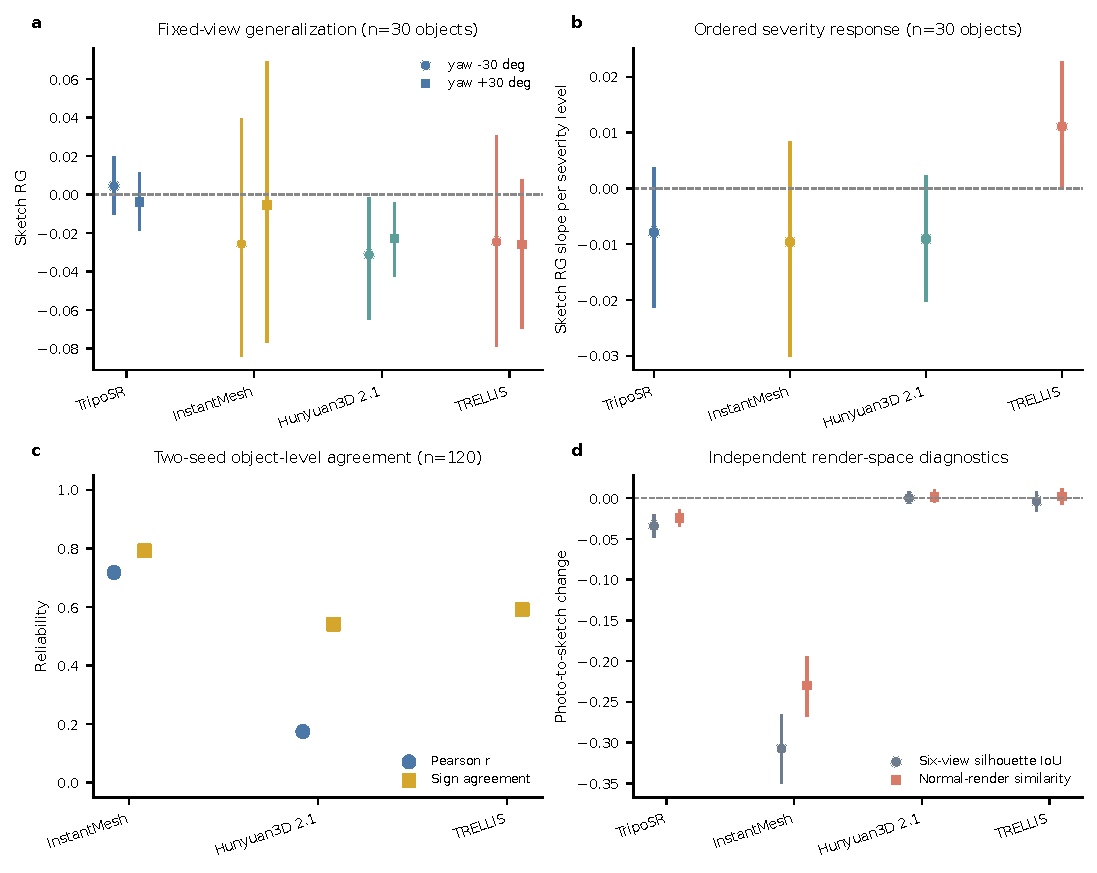
\includegraphics[width=\linewidth]{figures/fig4_confirmatory_robustness.pdf}
\caption{\label{fig:robustness}Robustness and independent diagnostics. (A) Sketch RG at two fixed additional views for V30. (B) Linear sketch RG slope across low, medium, and high abstraction severity in S30. (C) Object-level agreement between the two random seeds for stochastic models. (D) Photo-to-sketch change in independent six-view silhouette IoU and normal-render similarity. Error bars in A, B, and D are 99\% object-cluster bootstrap intervals.}
\end{figure}

Severity response was not monotonic in the direction predicted by the discovery hypothesis (Figure~\ref{fig:robustness}B). TripoSR, InstantMesh, and Hunyuan3D 2.1 had mean sketch RG slopes of $-0.0079$, $-0.0096$, and $-0.0091$ per severity level, respectively; their intervals crossed zero. TRELLIS alone had a positive slope, 0.0111, with 99\% CI $[0.0003,0.0226]$. For edge, TripoSR and InstantMesh had significantly negative slopes. A stronger visual abstraction can therefore worsen absolute geometry without necessarily increasing the surface--solid difference.

Seed reliability varied substantially (Figure~\ref{fig:robustness}C). InstantMesh object-level sketch RG had Pearson $r=0.718$, Spearman $\rho=0.701$, and 79.2\% sign agreement across seeds. Hunyuan3D 2.1 had Pearson $r=0.175$ and 54.2\% sign agreement. TRELLIS had Pearson $r=-0.253$ and 59.2\% sign agreement. Mean responses can be stable even when the same objects do not retain their rank or RG sign under another random draw. For a stochastic image-to-3D system, one output per input is therefore inadequate for object-level claims.

\subsection{Exploratory morphology associations}

Ground-truth morphology was most informative for InstantMesh. Its sketch RG correlated with solid volume ($\rho=0.598$), solidity ($\rho=0.549$), and bounding-box fill ($\rho=0.682$); all remained significant after within-model Holm correction. Objects that occupied more of their bounding box tended to show a larger solid-over-surface degradation difference. Hunyuan3D 2.1 showed a negative association with elongation ($\rho=-0.321$, corrected $p=0.00245$). TripoSR and TRELLIS had no association that survived within-model correction.

These analyses were exploratory and do not identify a causal mechanism. In particular, bounding-box fill may covary with category, visible-face area, or the stability of voxelisation. The result is best used to design a stratified follow-up benchmark. It does not support a claim that one morphological feature causes a model to fail.

\section{Discussion}

\subsection{The negative primary result changes the scientific claim}

The central finding is a rejection of the proposed universal sketch robustness gap. The discovery experiment suggested that artistic abstraction might systematically make surface F-score look more robust than solid occupancy. The larger, independent four-model test did not support that statement. TripoSR produced a small positive estimate that did not survive multiplicity correction; the other three models had intervals crossing zero. Only the model-by-style interaction passed the supporting gate.

This is not a reason to return to the smaller discovery claim. It is the reason for the present benchmark. A method or diagnostic that appears general in one fast baseline can fail when architectures, generation processes, and geometry decoders change. Reporting this result protects subsequent work from optimising against an artefact of model choice. It also yields a stronger practical statement: cross-style robustness cannot be assigned to \enquote{image-to-3D generation} as a single capability. It must be measured for a particular system, input depiction, random-seed policy, and evaluation threshold.

The result also distinguishes metric disagreement from geometric degradation. InstantMesh suffered the largest sketch failure in both F-score and IoU, yet its mean gap was modest because the two losses were similar. Hunyuan3D 2.1 and TRELLIS had near-zero sketch gaps because both mean changes were small. A positive RG is therefore neither necessary nor sufficient for a poor reconstruction. The main use of RG is diagnostic: it tells an evaluator when two metric families diverge. Absolute metrics and visual evidence still determine the severity of the failure.

\subsection{Implications for computational design}

Model selection for design tools often begins with natural-image demonstrations. Our results show why that evidence is incomplete. InstantMesh had the strongest photo baseline in this cohort but the largest degradation under sketch and edge input. Hunyuan3D 2.1 and TRELLIS were more stable for canonical sketches, although edge or low-detail input still reduced their geometry scores. A user who works primarily from line drawings could therefore prefer a system that is not the top photo-only baseline.

The appropriate screening test is small and paired. A design team can choose known objects that resemble its intended assets, render or collect matched photo and drawing conditions, and evaluate candidate systems with the same geometry target. Surface F-score, solid IoU, multi-view silhouettes, normal renders, connected components, and failure rate each add a different piece of evidence. The benchmark need not predict every artistic input. Its purpose is to expose whether the actual input convention of a workflow changes the relative ranking of available systems.

These diagnostics are relevant to downstream editing. Fragmented components complicate remeshing and rigging. Incorrect occupancy can make a rotated object appear thin or change how parts intersect. A source-view render can hide both problems. Six-view silhouette and normal comparisons are inexpensive checks before a mesh enters manual production. They do not measure aesthetic quality, but they help separate a recognisable source-view image from a geometrically coherent asset.

The benchmark also suggests a design requirement for future systems. Robustness should be evaluated across depiction families during development, not added as a final gallery. Training or preprocessing methods that translate sketches into photo-like cues may improve one model and damage another. A mitigation should therefore be tested against known ground truth and should report whether it changes surface, solid, topology, and render measures in the same direction. A visually more photographic input is not automatically a geometrically safer input.

\subsection{Implications for 3D benchmark design}

Recent benchmark and quality-assessment work has broadened the evaluation of generative 3D content \parencite{jiang2025threedgenbench,ebert2025threedarena,fu2025si23dcqa}. The present results add three recommendations. First, non-photographic input should be represented by matched perturbations when the research question concerns robustness. Without pairing, object and camera variation can dominate style. Second, benchmark reports should keep surface and solid changes separate before reducing them to a gap or composite score. Third, stochastic models need repeated seeds if conclusions are made at object level.

Threshold sensitivity deserves explicit reporting. The model-by-style interaction was compelling at $F_{0.05}$ and weaker at $F_{0.10}$. This does not invalidate either tolerance. It shows that a tolerance defines what counts as recovered surface and can change the balance between metric families. A benchmark that publishes only the favourable threshold invites over-interpretation. Reporting at least two tolerances, plus a threshold-free distance such as Chamfer, makes the dependence visible.

The failed gate also illustrates the value of freezing an evidence boundary without calling the study formally pre-registered. The protocol was recorded before confirmatory selection and inference, and discovery objects were excluded. This separation prevents a result-driven change in the primary style, metric, or multiplicity rule. Public registration would strengthen future work, especially if a benchmark comparison could influence model claims or commercial selection.

\subsection{Why systems respond differently}

The experiment was not designed to isolate internal mechanisms, so architectural explanations remain hypotheses. The four systems differ in image conditioning, generated-view use, 3D representation, training data, geometry decoding, and stochastic sampling. TripoSR reconstructs rapidly through a feed-forward triplane pipeline. InstantMesh relies on generated multi-view images before sparse-view reconstruction. Hunyuan3D 2.1 uses a high-resolution shape generation pipeline. TRELLIS generates structured 3D latents before mesh decoding. A sketch may therefore perturb an early view-generation stage in one system and be absorbed by a learned shape prior in another.

InstantMesh's combination of a strong photo baseline, large sketch/edge losses, high cross-seed RG correlation, and increased component count suggests a repeatable sensitivity in its pipeline rather than isolated numerical noise. By contrast, Hunyuan3D 2.1 and TRELLIS had low object-level seed reliability even where their mean canonical sketch changes were small. Their aggregate robustness may be produced by different objects improving and worsening across random draws. This distinction matters when a user needs one reliable asset rather than a favourable dataset average.

The morphology associations offer limited clues. Compact, high-fill objects had larger InstantMesh RG, while elongated objects had a more negative Hunyuan3D 2.1 RG. These patterns could reflect silhouette ambiguity, view generation, or voxel occupancy geometry. A mechanism study would need controlled primitive families, more camera views, intermediate model outputs, and interventions on shading or contour cues. The current evidence supports heterogeneity, not a causal account of it.

\subsection{Relation to specialised artistic 3D methods}

Specialised sketch and illustration methods aim to solve a different problem from this benchmark \parencite{sanghi2023sketchashape,zheng2024sketch3d,lee2025pasta,cong2025art3d}. They may encode stroke, part, or style priors that general-purpose systems lack. Our results should not be read as a ranking against those methods. Instead, the paired protocol offers a way to test whether a specialised method improves geometry because it understands the artistic input, rather than because its outputs look plausible from one view.

A useful next comparison would include a specialised sketch-to-3D method, a general model, and a style-normalisation front end on the same known objects. The endpoints should include absolute photo and sketch quality, paired degradation, topology, and a blinded human task. The human task should ask about recognisability under rotation, editability, part integrity, and preference for downstream use. It should not ask raters to score unrelated original and generated images as though they were paired.

\section{Limitations}

The benchmark has clear scope limits. The 120 objects are scanned household items from GSO. They do not represent characters, plants, vehicles, architecture, thin structures, or free-form industrial concepts in equal measure. The hash-ranked selection and strict solid audit reduce selection bias within the available source, but they do not create a universal object distribution. Category-stratified replication on other public datasets is needed.

The artistic conditions are controlled proxies. They preserve exact foreground support and camera, which is valuable for attribution, but real sketches and paintings do not. Human drawings can alter perspective, proportions, topology, part placement, and semantic emphasis. Watercolour can include paper texture and deliberate colour bleeding. A model that is stable under our deterministic sketch transform may still fail on novice drawings or expressive concept art. Controlled and real-art evaluations should be treated as complementary.

The study evaluates four open systems at frozen revisions and one geometry-oriented configuration per system. It does not evaluate proprietary services, newer checkpoints, texture pipelines, prompt-based refinement, or style-specific tuning. Hunyuan3D 2.1 was evaluated in shape-only mode even though its broader pipeline supports physically based materials. TRELLIS produced mesh output without using other decoders. These choices keep geometry comparison tractable but do not cover the full capability of each system.

The fixed model-level alignment avoids per-sample scale fitting, but any alignment convention influences point and voxel scores. We address this by calibrating on excluded discovery objects and adding render-space diagnostics. Additional work could report camera-aware unaligned measures or category-specific physical scale where available. Voxel IoU also depends on grid resolution and extent; a multi-resolution occupancy analysis would quantify that sensitivity.

Only two seeds were used for stochastic main runs, and V30/S30 used one seed for cost control. Two seeds are enough to reveal weak object-level reliability but not to estimate a full output distribution. The V30 and S30 subsets contain 30 objects, so their intervals are correspondingly broad. Their role is to limit generalisation of the canonical result, not to establish a definitive view or severity law.

No human usability scores are reported. Surface, solid, topology, and render diagnostics measure geometric properties, not whether an artist would accept, edit, or prefer an asset. We deliberately avoid treating those metrics as human judgement. A subsequent study should use matched cases from this benchmark, a blinded interface, multiple raters, and pre-defined agreement and exclusion rules.

Finally, the discovery-to-confirmation split was frozen locally but not registered in an external repository before inference. The timestamped protocol, schedules, hashes, code revisions, complete job records, and failed gate make the analysis auditable, but a public prospective registration would provide stronger protection against undisclosed flexibility.

\section{Conclusion}

We evaluated 120 known 3D objects under one photo-like and five matched abstract depictions using TripoSR, InstantMesh, Hunyuan3D 2.1, and TRELLIS. The 6,240 completed reconstructions show that cross-style robustness is not a single property shared by current image-to-3D systems. The pre-specified sketch surface--solid gap failed in all four models after Holm correction. At the same time, model-by-style interaction was strong, and absolute losses ranged from negligible canonical-sketch changes in Hunyuan3D 2.1 and TRELLIS to severe surface, occupancy, topology, and six-view degradation in InstantMesh.

The practical conclusion is narrower and more defensible than the discovery-stage hypothesis. Photographic performance does not determine robustness to sketches or illustrations, and a near-zero metric gap does not certify good geometry. Computational-design evaluations should pair the same object across input depictions, report surface and solid fidelity separately, include multi-view and topology checks, and repeat stochastic inference when object-level reliability matters. The benchmark and its failed primary gate provide a reproducible basis for that evaluation rather than a universal claim about artistic input.

\section*{Conflicts of interest}

The authors declare no competing interests.

\section*{Author contributions}

Wei Xiong: Conceptualization, Methodology, Software, Validation, Formal analysis, Investigation, Data curation, Visualization, Writing--original draft. Wei Meng: Methodology, Validation, Formal analysis, Investigation, Writing--review \& editing. Chu Qiu: Conceptualization, Resources, Supervision, Project administration, Writing--review \& editing. ShuWen Li: Data curation, Validation, Investigation, Visualization, Writing--review \& editing. Zhanhao Liang: Supervision, Writing--review \& editing. All authors reviewed and approved the final manuscript.

\section*{Funding}

This research received no specific grant from any funding agency in the public, commercial, or not-for-profit sectors.

\section*{Data availability}

Google Scanned Objects is publicly described and linked on the \href{https://research.google/pubs/google-scanned-objects-a-high-quality-dataset-of-3d-scanned-household-items/}{Google Research dataset page}. The submission package contains the frozen protocol, confirmatory schedules, selected-object manifest, code revisions, evaluation and analysis scripts, aggregate object-level tables, figure-generation code, representative-case rule, and validation report. Source assets are identified rather than redistributed and remain subject to their source terms. The complete auditable package will be deposited in a persistent public repository before publication; during peer review it is available from the corresponding authors.

\printbibliography

\end{document}
